% CARPK 성능 테이블
\begin{table}[t!]
    \small
    \setlength{\extrarowheight}{2.3pt}
    \setlength{\tabcolsep}{1.5pt}
    \centering
    
    \begin{tabular*}{\linewidth}{l@{\extracolsep{\fill}}*{4}{c}}
    
    \hline
    \multirow{2}{*}{Methods} & \multicolumn{2}{c}{CARPK} & \multicolumn{2}{c}{PUCPR+} \\
    \cline{2-3}\cline{4-5}
    & MAE & RMSE & MAE & RMSE \\
    
    % Few-shot
    \hline
    \textbf{\textit{few-shot}} & & \\
    FamNet & 28.84 & 44.47 & 87.54 & 117.68 \\
    BMNet & 14.61 & 24.60 & 103.18 & 112.42 \\
    BMNet+ & 10.44 & 13.77 & 62.42 & 81.74  \\
    
    % Zero-shot
    \hline
    \textbf{\textit{zero-shot}} \\
    VLBase & 20.47 & 24.33 & 90.82 & 104.01 \\
    VLCounter & \textbf{6.46} & \textbf{8.68} & \textbf{48.94} & \textbf{69.08} \\
    \hline
    
    \end{tabular*}
    
    \caption{Cross-dataset validation performance on the CARPK and PUCPR+ dataset.}
    \label{tab:CARPK}
\end{table}
\section{Experiments}

In this section, we provide a comprehensive explanation of experimental details.
First, we delve into the implementation details, datasets, and evaluation metrics in Sec.~5.1, followed by a comparison of our model with existing state-of-the-art methods in Sec.~5.2.
Then, we conduct an in-depth exploration of each component further in Sec.~5.3.


\subsection{Experimental Details}

\paragraph{Implementation Details.}
For all experiments, we employed CLIP ViT-B/16 as our encoders followed by a decoder consisting of 4 repeated units.
Each of these units consists of one feature projection block in Fig.~\ref{fig:SaSC} and one additional convolutional layer.
Regarding the image input, each image is resized to $384\times384$, and augmentations such as gaussian noise, gaussian blur, horizontal flip, and color jittering were applied.
We trained the model using AdamW~\cite{2017adamw} optimizer with a learning rate of $1\mathrm{e}^{-4}$ and weight decay of $1\mathrm{e}^{-2}$ for 200 epochs with a batch size of 16 on a single NVIDIA RTX A6000.
For temperature scaling and loss-balancing hyperparameter $\lambda$ and $\tau$, we used $1\mathrm{e}^{-6}$ and 1.


\paragraph{Datasets.}
To explore the counting capability of models, we use FSC147~\cite{2021FAMNet}, the first large-scale dataset for class-agnostic counting.
It includes 6135 images from 147 categories mainly composed of foods, animals, kitchen utensils, and vehicles.
We also utilize CARPK and PUCPR+~\cite{2017drone} datasets.
These datasets exhibit different properties from the images in FSC147, so we use them for cross-dataset validation which is to test the model's generality.
To be specific, CARPK consists of 1,448 parking lot images with nearly 90,000 cars taken in a drone view at 40 meters height on average.
On the other hand, PUCPR+ contains nearly 16,456 cars in total which have 10th-floor-view images.


\begin{table}[t]
    \small
    \setlength{\extrarowheight}{2.3pt}
    \setlength{\tabcolsep}{1.5pt}
    \centering
    
    \begin{tabular*}{3.3in}{@{\extracolsep{\fill}}*{8}{c}}

    % Valid
    \hline
    \multirow{2}{*}{No.} & \multirow{2}{*}{SPT} & \multirow{2}{*}{LAT} & \multirow{2}{*}{SaSC} & \multicolumn{2}{c}{Val set} & \multicolumn{2}{c}{Test set} \\
    \cline{5-6}\cline{7-8}
    & & & & MAE & RMSE & MAE & RMSE \\
    \hline
    M1 & $\times$ & $\times$ & $\times$ & 31.82 & 98.89 & 32.20 & 130.51 \\
    M2 & \checkmark & $\times$ & $\times$ & 20.61 & 75.36 & 17.58 & 112.89 \\
    M3 & $\times$ & \checkmark & $\times$ & 29.97 & 96.59 & 28.26 & 127.44 \\
    M4 & $\times$ & $\times$ & \checkmark & 24.88 & 81.28 & 24.16 & 113.01 \\
    M5 & \checkmark & \checkmark & \checkmark & \textbf{18.06} & \textbf{65.13} & \textbf{17.05} & \textbf{106.16} \\
    \hline
    
    \end{tabular*}    
    \caption{  
        Ablation study on each component of VLCounter.
        % Ablation study to analyze the components of VLCounter. 
        % Ablation study on learnable affine transform~(LAT), text conditioned prompt tuning~(TPT), and similarity-aware skip connection~(SaSC).
    }
    \label{tab:ablation}
\end{table}


% \paragraph{Evaluation Metrics.} 
% For a fair comparison, we adopt Mean Average Error~(MAE) and Root Mean Squared Error~(RMSE) to evaluate the performances following the conventions of previous works~\cite{2022BMNet, 2021FAMNet, 2023zsc, 2022RepRPN}.


\subsection{Comparison with State-of-the-art Methods}
We compare VLBase and VLCounter against previous class-agnostic counting methods in Tab.~\ref{tab:main}.
Despite its simple design, the performances of VLBase are comparable to the two-stage methods that even utilize additional training data.
% For VLBase, although its simplicity in its design choice and pipeline, we find its performances are comparable to the two-stage methods that utilize additional training data.
On the other hand, VLcounter clearly surpasses other ZSOC baselines.
Particularly, when compared to ZSC, VLCounter achieves a relative improvement of 32.94\% and 22.81\% in terms of validation MAE and test MAE, respectively.
Moreover, we remark on the comparable results to the state-of-the-art few-shot counting method: BMNet.
This is an especially notable milestone for ZSOC since few-shot methods are generally seen as the upper bound of two-stage ZSOC methods; the counting framework in two-stage works is usually adopted from few-shot methods.

On the rightmost columns, we provide the inference speed per image.
% On the rightmost columns, we mention the number of learnable parameters and inference speed per image.
As our one-stage approaches~(VLBase and VLCounter) only require the time to count the objects, it is shown that their inference speeds are much f   aster than a two-stage method~(ZSC) which needs extra time to discover exemplars~(denoted as $\alpha$ since the implementation is not fully publicized).
In addition to the inference time, VLBase and VLCounter have much fewer parameters to learn, having their strength in shorter training time~(Training time for VLCounter is approximately 2$\times$ faster than BMNet+).


Following previous class-agnostic counting methods~\cite{2021FAMNet, 2022BMNet}, we verify the generalization capability of VLBase and VLCounter by conducting a cross-dataset evaluation on CARPK and PUCPR+ datasets in Tab.~\ref{tab:CARPK}, and VLBase and VLCounter demonstrate their benefits in generalization.
Whereas the performance gaps between few-shot methods and VLBase is reduced, we observe the superiority of VLCounter to other methods by boosting MAE up to 38.12\% and 27.54\% in CARPK and PUCPR+ datasets compared to BMNet+.
In particular, we emphasize the single-digit results of VLCounter in terms of both MAE and RMSE are derived without any fine-tuning~(The average number of cars in each image of CARPK is 62).
We attribute such success in cross-dataset validation to adapting the generality of CLIP to counting-specific and incorporating multi-level features to provide rich semantics into the prediction, each approximately taking 54\% and 46\% portions in the increase in CARPK MAE.



\subsection{Ablation Studies on VLCounter}
\paragraph{Component Analysis.}
To validate the effectiveness of individual components, we conducted an ablation study as presented in Tab.~\ref{tab:ablation}.
% To validate the effectiveness of individual components, we conducted an ablation study in Tab.~\ref{tab:ablation}.
Starting with VLBase~(M1), we add SPT, LAT, and SaSC in M2, M3, and M4, respectively.
Among the individual components, the effectiveness of SPT demonstrated in M2 is the most pronounced.
% The effectiveness of SPT shown in M2 is the best of the individual component. 
This significant improvement demonstrates the importance of fine-tuning incorporated with the semantic condition.
LAT in M3 is another important component.
While it can be seen as not incurring a dramatic increase in performance, the counting map $\hat{S}$ derived from LAT is also an essential element in SaSC.
Lastly, M4 shows that SaSC not only boosts generalization capability but also task-specific predictions.
This is because layer-wise intermediate representations in CLIP encoder are also semantically meaningful~\cite{li2023clipsurgery} and SaSC aggregates them to aid counting prediction.

% 컴포넌트 Ablation
\begin{table}[t]
    \small
    \setlength{\extrarowheight}{2.3pt}
    \setlength{\tabcolsep}{1.5pt}
    \centering
    \begin{tabular*}{\linewidth}{l@{\extracolsep{\fill}}*{5}{c}}
    \hline
    \multicolumn{2}{c}{\multirow{2}{*}{Condition}} & \multicolumn{2}{c}{Val set} & \multicolumn{2}{c}{Test set} \\
    \cline{3-4}\cline{5-6}
     & & MAE & RMSE & MAE & RMSE \\
    \hline
    \multicolumn{2}{c}{VLCounter} & 18.06 & 65.13 & 17.05 & 106.16 \\ \hline
    \textbf{SPT} & w/o $\mathcal{T}'$ & 19.07 & 65.72 & 17.19 & 107.54 \\
    % w/ $\mathcal{T}'$ & 18.06 & 65.13 & 17.05 & 106.16 \\
    \hline
    \textbf{SaSC} & w/o $\hat{S}$ & 20.28 & 65.54 & 19.38 & 105.69 \\
    % \textbf{SaSC} & w/ $S$ & 18.30 & 61.60 & 17.72 & 105.19 \\
    % w/ $C$ & 18.06 & 65.13 & 17.05 & 106.16\\
    \hline
    % \hline
    \end{tabular*}
    \caption{Analysis of semantic-conditioning techniques in SPT and SaSC.}
    \label{tab:ablation_component}
\end{table} 

\begin{table}[t]
    \small
    \setlength{\extrarowheight}{2.3pt}
    \setlength{\tabcolsep}{6pt}
    \centering
    % \begin{tabular}{ccccc}
    \begin{tabular*}{0.9\linewidth}{@{\extracolsep{\fill}}*{5}{c}}

    \hline
    \multirow{2}{*}{Text prompts} & \multicolumn{2}{c}{Val set} & \multicolumn{2}{c}{Test set} \\
    \cline{2-3}\cline{4-5}
     & MAE & RMSE & MAE & RMSE \\
    \hline
    Singular & 20.08 & 67.92 & 19.18 & 105.04 \\
    \hline
    Plural & 18.06 & 65.13 & 17.05 & 106.16 \\ 
    \hline
    \end{tabular*}
    \caption{Analysis of pluralized context to prompt the class names.}
    \label{tab:ablation_plural}
\end{table} 

\paragraph{Effect of conditioning semantic information.}
%In this subsection, 
We further conduct ablation studies on semantic conditioning.
In Tab.~\ref{tab:ablation_component}, we compare conventional VPT with SPT and test the semantic conditioning in SaSC.
Along with the benefits of VPT of granting task-specificity, utilizing semantic conditions in VPT allows the prompts to be more semantically specific.
In addition, using semantic conditions in filtering the knowledge that is passed to the decoder with residual paths clearly benefits SaSC. 
We think that the semantic conditioning with the counting map $\hat{S}$ suppresses the object-irrelevant information, thereby contributing to the improvements.



% 정성 평가 결과 그림
\begin{figure*}[t]
    \begin{center}
        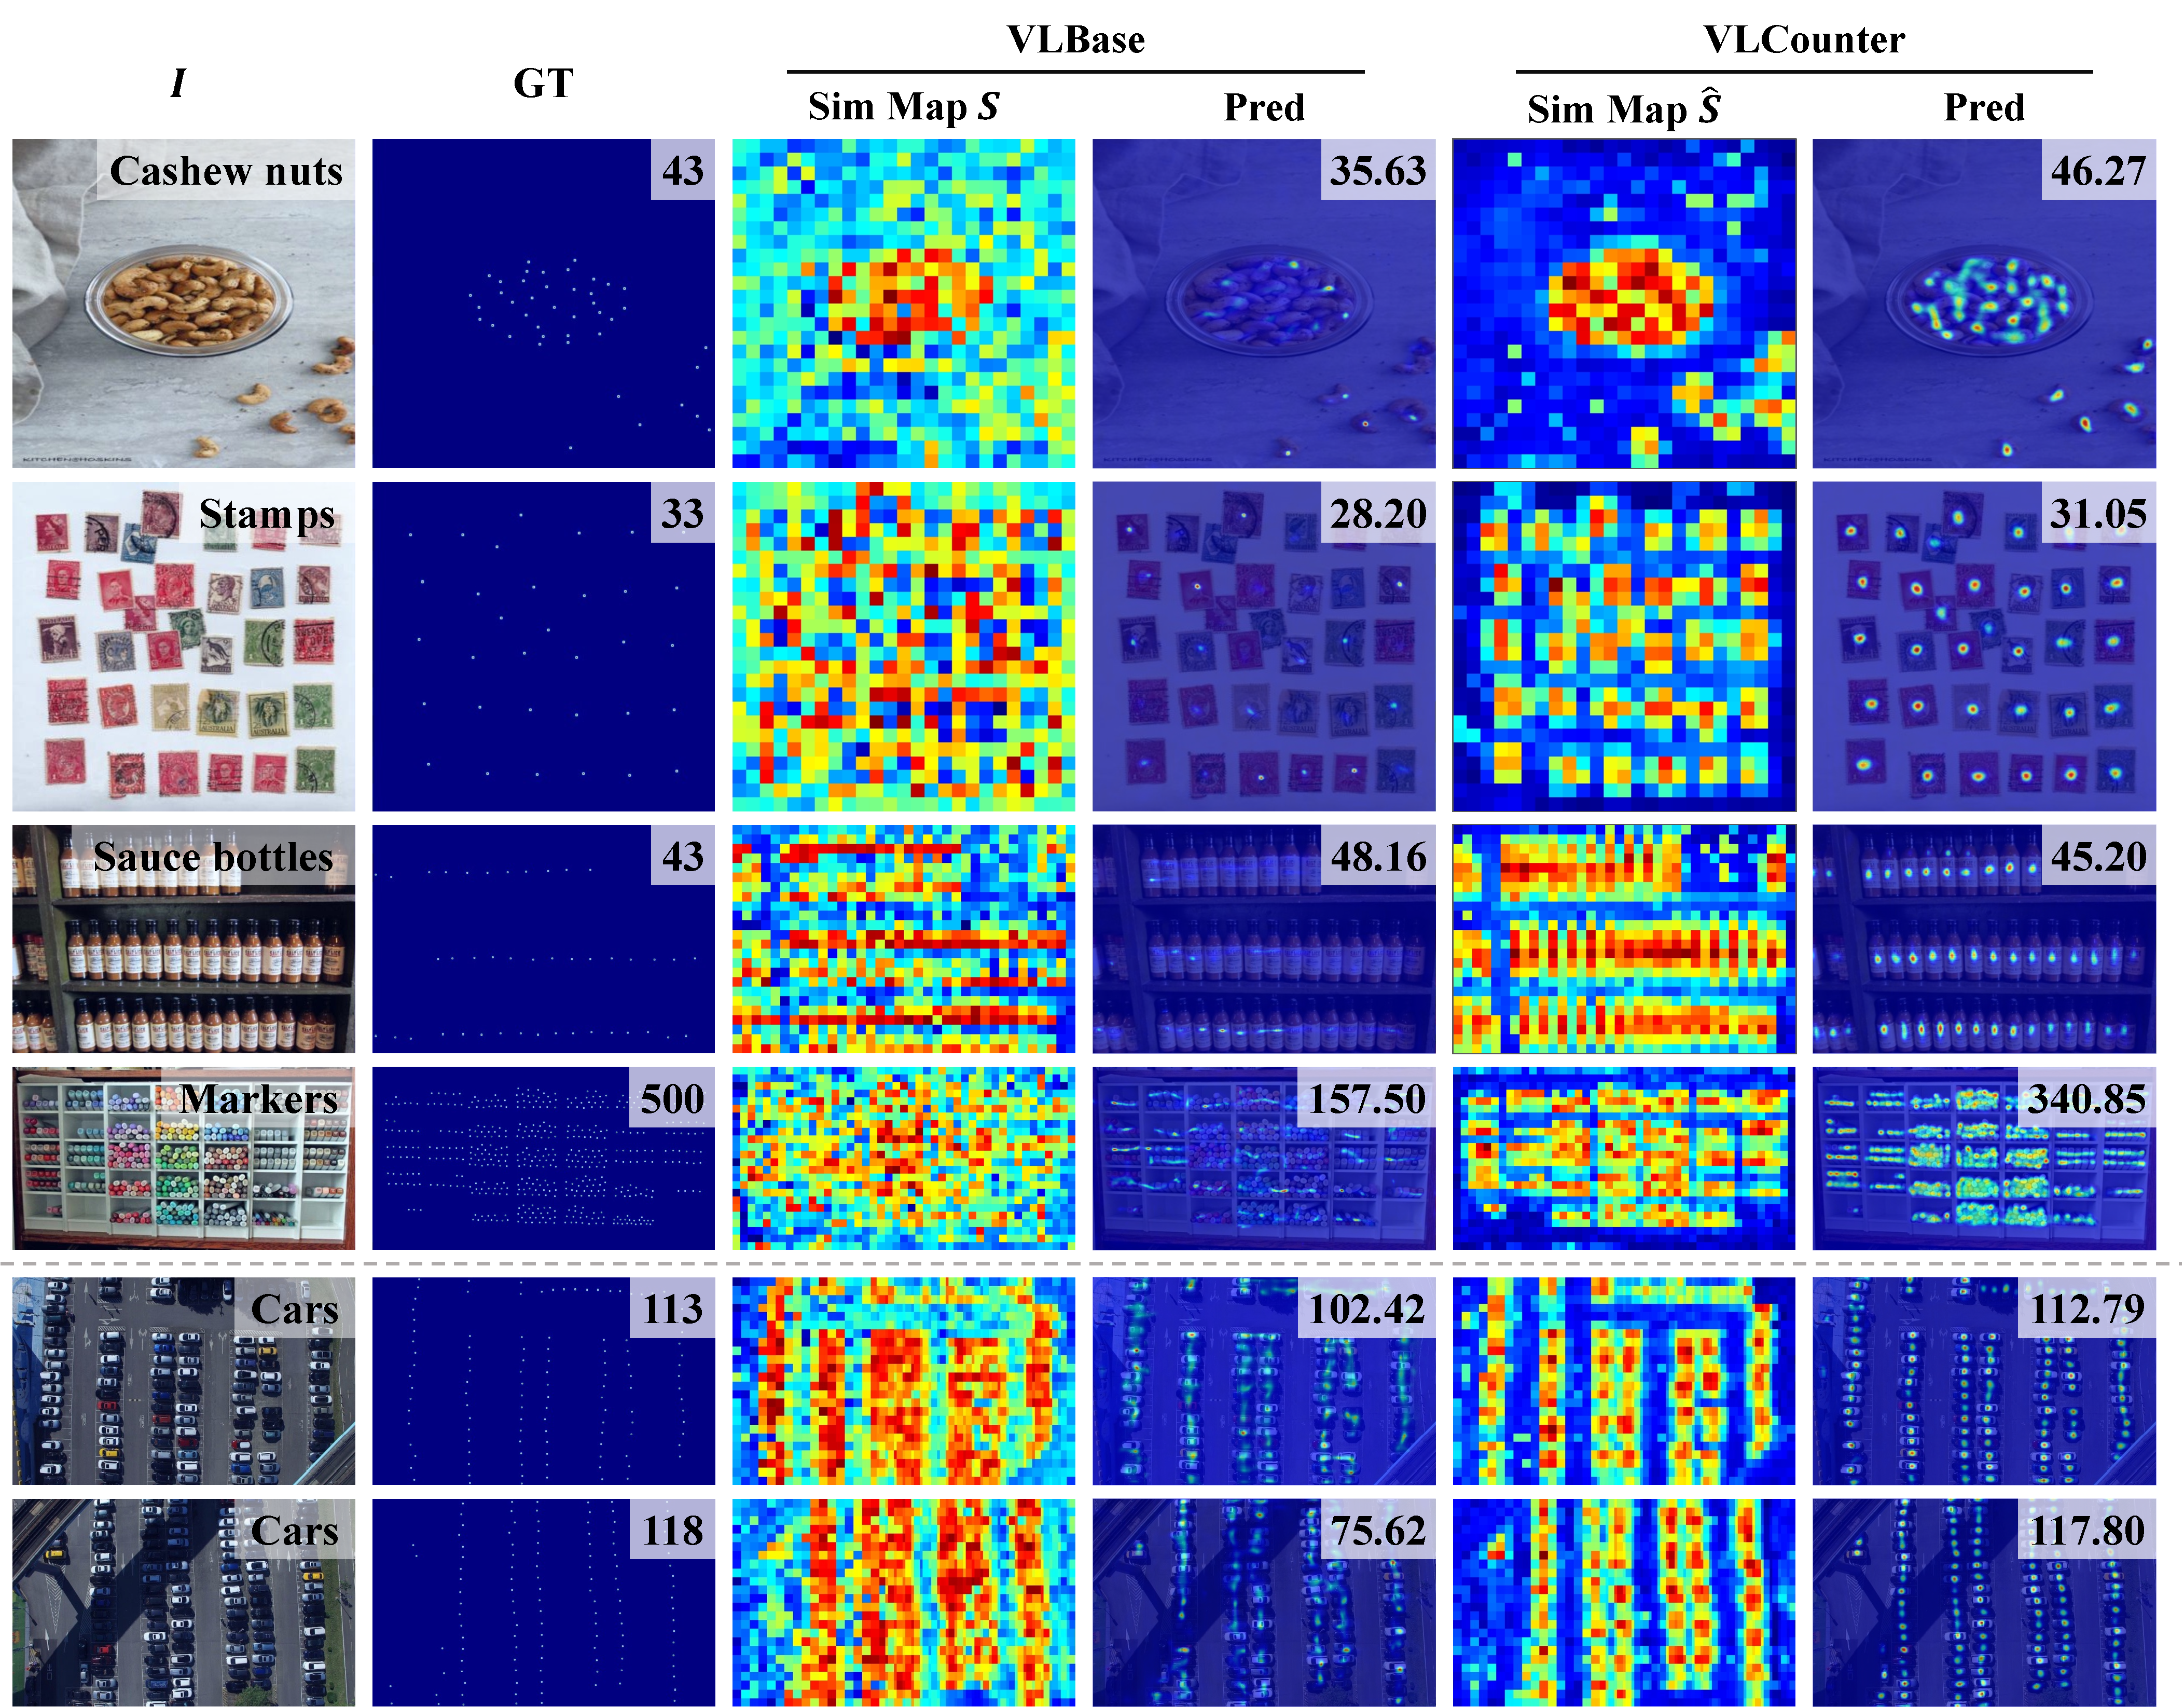
\includegraphics[width=0.95\linewidth]{figs/qualitative.pdf}
    \end{center}
    \caption{
        Qualitative comparison of VLBase and VLCounter on the FSC-147~(Top 4 rows) and CARPK~(Bottom 2 rows).
        Class names and counting values are shown at the right top of the query image~($I$) and the predicted density map, respectively.
    }
    \label{fig:qualitative_results}
\end{figure*}


\paragraph{Effect of plural text prompts.}
We followed CLIP~\cite{2021clip} to use different context prompts to encode the semantic embeddings.
Yet, since the counting task mainly assumes the existence of multiple instances in every image, we modified text prompts to be in plural form.
In Tab.~\ref{tab:ablation_plural}, we compare the results between using singular and plural forms of text prompts, and text prompts in plural form have the advantage in the counting task.




\subsection{Qualitative Results}
Along with the quantitative results, we study how the components of VLCounter affect class-specificity.
In Fig.~\ref{fig:qualitative_results}, we compare both the similarity map and the density map of VLBase and VLCounter.
By delivering the semantic condition and fine-tuning the similarity map, we find the similarity map to retain more compact salient regions; the activations in the background are suppressed~(1st, 2nd rows) and object regions are clearly localized~(2nd, 3rd rows).
Then, by aggregating multi-level representations of rich semantics with these similarity maps in the decoder, we observe the clear discrepancy between the predicted density maps from VLBase and VLCounter, especially for densely populated images~(4th row). 





Furthermore, we provide the cross-dataset results in the last two rows in Fig.~\ref{fig:qualitative_results}.
Similar to what we discussed with predictions for FSC147, we verify that VLCounter is a counting-tailored and generalizable model across new categories, shapes, and densities of objects.
These results verify the advantage of employing a pretrained vision-language model for capturing the semantics of newly seen objects, i.e., cars.
% With.... and SaSC that passes generalization capability to the decoder via multiple connections, we validate the robustness of VLCounter across new categories, shapes, sizes, and densities of objects.
Refer to the appendix for more visualizations.

